\documentclass[12pt,letterpaper]{article}

\usepackage{tikz}
\usetikzlibrary{shapes}

\usepackage{amssymb,amsmath,amsthm}
\usepackage{enumerate}
\usepackage[margin=1.25in]{geometry}
\usepackage{graphicx,ctable,booktabs}
\usepackage{fancyhdr}
\usepackage[utf8]{inputenc}
\usepackage{gensymb}
\usepackage{wrapfig}

\makeatletter
\newenvironment{problem}{\@startsection
       {section}
       {1}
       {-.2em}
       {-3.5ex plus -1ex minus -.2ex}
       {2.3ex plus .2ex}
       {\pagebreak[3]
       \large\bf\noindent{Problem }
       }
       }
\makeatother

\title{Quadrilaterals}
\author{Name: \underline{\hspace{5cm}}}
\date{April 24, 2015}

\pagestyle{fancy}
\lhead{Quadrilaterals}
\chead{} 
\rhead{\thepage} 
\lfoot{\small\scshape Grade 4 Olympic Math} 
\cfoot{} 
\rfoot{}
\renewcommand{\headrulewidth}{.3pt} 
\renewcommand{\footrulewidth}{.3pt}
\setlength\voffset{-0.25in}
\setlength\textheight{648pt}
\setlength\headheight{15pt}

\begin{document}

\maketitle

\thispagestyle{empty}

\begin{problem}{Area of a Triangle}
 Complete the table for each triangle.
 
 \begin{center}
 \begin{tabular}{|c|c|c|}
  \hline
  Base & Height & Area \\
  \hline
  $10$ & $20$ & \\
  $15$ & $8$ & \\
  & $10$ & $60$ \\
  & $14$ & $49$ \\
  $5$ & & $15$ \\
  $20$ & & $100$\\
  \hline
 \end{tabular}
 \end{center}
\end{problem}

\begin{problem}{Area of a Parallelogram}
 Complete the table for each parallelogram.
 
 \begin{center}
 \begin{tabular}{|c|c|c|}
  \hline
  Base & Height & Area \\
  \hline
  $7$ & $8$ & \\
  $15$ & $4$ & \\
  $5$ & & $50$ \\
  & $3$ & $36$ \\
  $20$ & $3$ & \\
  \hline
 \end{tabular}
 \end{center}
\end{problem}

\begin{problem}{Rectangle}
 Circle ``True'' or ``False'' for each statement.
 \begin{itemize}
  \item All rectangles are parallelograms. \hfill True~~False
  \item All rectangles are squares. \hfill True~~False
  \item The interior angles of all rectangles sum to $360\degree$. \hfill True~~False
  \item Rectangles always have $4$ obtuse angles. \hfill True~~False
 \end{itemize}
\end{problem}

\begin{problem}{Area of a Rectangle}
 Find the area of each rectangle.

 \begin{center}
 \begin{tabular}{|c|c|c|}
  \hline
  Width & Length & Area \\
  \hline
  $10$ & $5$ & \\
  $8$ & $12$ & \\
  \hline
 \end{tabular}
 \end{center}
\end{problem}

\begin{problem}{Trapezoid}
 Circle ``True'' or ``False'' for each statement.
 \begin{itemize}
  \item All trapezoids are parallelograms. \hfill True~~False
  \item All parallelograms are trapezoids. \hfill True~~False
  \item Trapezoids have at least one set of perpendicular sides. \hfill True~~False
  \item The area of a trapezoid depends on its height. \hfill True~~False
 \end{itemize}
\end{problem}

\begin{problem}{Area of a Trapezoid}
 Find the area of each trapezoid.

 \begin{center}
 \begin{tabular}{|c|c|c|c|}
  \hline
  Upper base & Lower base & Height & Area \\
  \hline
  $5$ & $7$ & $5$ & \\
  $8$ & $12$ & $17$ & \\
  \hline
 \end{tabular}
 \end{center}
\end{problem}

\begin{problem}{Challenge}
 What's the area of this kite? (The diagonals [dotted lines] measure $30$ and $50$ and intersect at right angles.)
 
 \begin{figure}[h]
 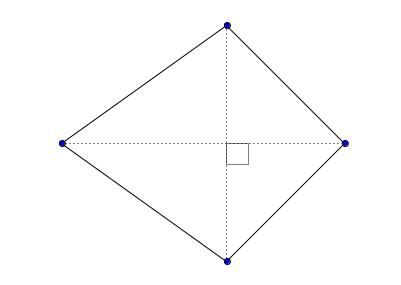
\includegraphics[width=250px]{kite.png}
 \end{figure}
\end{problem}


\end{document}